\chapter{Conception}


%% ------------------------------------------ %%
%%               ARCHITECTURE                 %%
%% ------------------------------------------ %%
\section{Architecture du système}\label{conception.architecture}

\subsection{Architecture logique}

\todo{VM, etc.}

\subsection{Architecture physique}
\subsubsection{Connexion de la caméra}\label{conception.architecture.physique.camera}
\todo{Schéma des différentes connexions possible + choix}

\subsubsection{Réseau}
\todo{Schéma réseau physique}


\todo{Architecture choisie : sur le toit, construction d'une salle en cours --> panneau solaire}

%% ------------------------------------------ %%
%%           CHOIX TECHNOLOGIQUES             %%
%% ------------------------------------------ %%

\section{Choix technologiques}

\subsection{Caméra réseau}
Une caméra réseau fournissant des images de qualités, et ce dans un prix raisonable, est nécessaire dans ce projet afin de capturer des images. 

\subsubsection{Contraintes}\label{conception.techno.camera.contraintes}
Installer une caméra sur le toit de la HEIG-VD a pour conséquence que certaines contraintes, tant d'ordre techniques qu'organisationnelles, doivent être respectées. Celles-ci sont décrites dans cette section.

\paragraph{Capture de photo}
La caméra devra au minimum permettre la capture de photos à intervalles réguliers d'une façon ou d'une autre. La capture de vidéos n'est pas nécessaire.  On notera que si celle-ci ne fournit malheureusement que la fonctionnalité de capture vidéo, il serait tout de même possible d'en extraire des images utilisables. 

\paragraph{Usage extérieur}
La caméra doit être prévue pour un usage extérieur, avec une protection contre les intempéries (pluie, neige, froid, chaud, etc.).

\paragraph{Connexion réseau}
En lien avec le paragraphe précédent, la caméra doit nécessairement avoir une interface Wifi permettant de se connecter au réseau de l'école. Une connexion par Ethernet n'est pas envisageable.

\paragraph{Caméra auto-alimentée}
Comme vu en section \ref{conception.architecture.physique.camera}, la caméra doit être auto-alimentée et non cablée. Ainsi, une combinaison de batteries et de panneaux solaires semble être idéal. On peut noter que l'utilisation de batteries uniquement est envisageable dans le cadre d'un prototypage, mais ce uniquement si le remplacement de celles-ci doit être effectué à intervalles relativement éloignés, de l'ordre de la semaine.

\paragraph{Résolution d'image}
Dans le but d'obtenir des images de qualités suffisantes, la résolution de l'image capturées devra nécessairement être d'au minimum 1280x720 pixels.

\subsubsection{Critères}
Plusieurs critères, ont été définis. Chacune des caméras retenues seront notées selon ceux-ci. On les trouvera ci-après, où leur pondération sont indiqués entre crochets ([]). Une pondération élevée signifie une plus grande importance de ce critère.

\paragraph{Qualité d'image [1]}
La caméra doit avoir une bonne qualité d'image. On jugera:
\begin{itemize}
    \item La résolutions de l'image. Celle-ci doit être d'au minimum 1280x720 pixels.
    \item La qualité de l'image (si possible).
\end{itemize}

\paragraph{Fonctionnalités réseaux [2]}
La caméra doit pouvoir fournir des images via le réseau et il doit être possible d'en récupérer à intervalles réguliers. Pour ce faire, on pensera à des protocoles comme les suivants: 
\begin{description}
    \item[ONVIF (Open Network Video Interface Forum)] Standard industriel ouvert permettant de contrôler, configurer et communiquer avec des caméras de sécurité IP. Permet notamment la lecture de flux vidéo en temps réel et la capture de photos \autocite{wiki:onvif}
    \item[RTSP (Real Time Streaming Protocol)] Développé par RealNetworks, Netscape et Clumbia UNiversity, protocole de communication permettant de lire en temps réel un flux vidéo. \autocite{wiki:RTSP}
    \item[Requêtes HTTP] Il pourrait être possible de capturer et de récupérer à la demande une photo à l'aide de requêtes HTTP.
    \item[Flux sur HTTP] Permet la lecture de flux vidéo sur HTTP en s'appuyant sur des formats tel que MPEG-4.
    \item[Interface Web HTTP] Permet la configuration de la caméra IP via un serveur Web qu'elle expose. 
    \item[FTP] La caméra peut exposer un serveur FTP contenant les photos capturées. Elle pourrait aussi téléverser des photos capturées sur un serveur FTP distant.
On notera avant tout sur la facilité d'utilisation des différents protocoles.
\end{description}

\paragraph{Fonctionnement auto-alimenté [4]}
La caméra doit être auto-alimentée et non cablée. Comme critères, on pensera donc à:
\begin{itemize}
    \item La durée de vie de la caméra en fonctionnement auto-alimenté. Idéalement, la caméra ne devrait nécessiter aucune intervention humaine.
    \item La portée du Wifi. La puissance du signal doit être assez forte afin de pouvoir capter les bornes Wifi de l'école depuis le toit de la HEIG-VD. Il est important de noter que ce critère peut être difficilement évalué avant l'achat de la caméra.
\end{itemize}

\paragraph{Capture de photo [2]}
La caméra doit être capable de fournir un moyen pour capturer des photos à intervalles réguliers. Pour ce faire, la caméra peut fournir un système de capture de photos automatique, ce qui est un plus. On évaluera donc les moyens fournis par la caméra permettant ces captures.

\paragraph{Angle de vue [2]}
L'angle de vue de la caméra doit être suffisamment grand afin d'obtenir une image du parking dans son ensemble. Il peut être suffisant à partir de 40°, de par la hauteur à laquelle elle sera placée. Cependant, un angle de 90° semble plus satisfaisant. Ces angles ont été définis à l'aide des informations fournies par \url{videosurveillance-boutique.fr} \autocite{cam:securite_info}.

\paragraph{Vision de nuit [1]}
Idéalement, la caméra devrait pouvoir fournir une vision de nuit afin de pouvoir capturer des images de parking par toute heure. On pensera notamment aux matinées et aux soirées d'hiver, où les véhicules arrivent et partent alors que la luminosité est encore très faible. Cependant, dans le cadre de ce TB, cette fonctionnalité n'est pas strictement nécessaire.

\paragraph{Facilité d'installation [1]}
La facilité d'installation de la caméra sera prise en compte. On pensera aux dimensions de celle-ci, à son poids, au nombre de ses composants (par exemple, est-il nécessaire d'installer une batterie en plus de la caméra, ou est-elle incorporée à celle-ci?), ou encore aux accessoires fournis pour son installation. 

\paragraph{Prix [2]} Bien évidemment, le prix doit entrer en ligne de compte. 100.- CHF sera indiqué comme prix maximum afin d'obtenir la meilleure note. A partir de 500.- CHF, on évaluera ce prix comme étant mauvais.

\subsubsection{Caméras disponibles et évaluation}
Bien que la surveillance n'est pas un but de ce TB, les caméras de sécurités semblent être les plus adaptées. En effet, elles fournissent généralement des fonctionnalités de capture de photos, de connexion réseau, de vision de nuit, possèdent un angle de vue suffisant et sont souvent résistantes à un environnement extérieur. De plus, elles sont spécialement concues pour un usage qui s'apparente à celui qui de ce TB, et sont donc adaptées à la prise d'images de parking.

L'achat distinct d'une caméra, de panneaux solaires et de batteries est envisageable. Néanmoins, dans un premier temps, seuls des kits complets (caméra, batteries, panneaux solaires) ont été analysés. En effet, l'installation et le choix des différents composants nécessaires à un système solaire complet semble difficile lorsqu'on est pas du domaine, et des problèmes d'interopérabilité pourraient survenir. Ceci reste cependant une solution viable si aucun kit ne correspond aux contraintes définies.

De part les contraintes très spécifiques précisées jusqu'ici, le nombre de caméras les satisfaisant toutes sont peu nombreuses. On trouvera ci-après les kits complets solaires auto-suffisants qui ont été évalués. Il faut aussi noter que seules les caméras les plus appropriées sont indiquées ici.

\paragraph{\textbf{Electrosun} -- Caméra-surveillance-solaire}
\textit{Electrosun} est une entreprise de domotique solaire française. Entre autres, un kit solaire de caméra complet est mis en vente. \autocite{cam:electrosun_site}

\begin{figure}[h]
    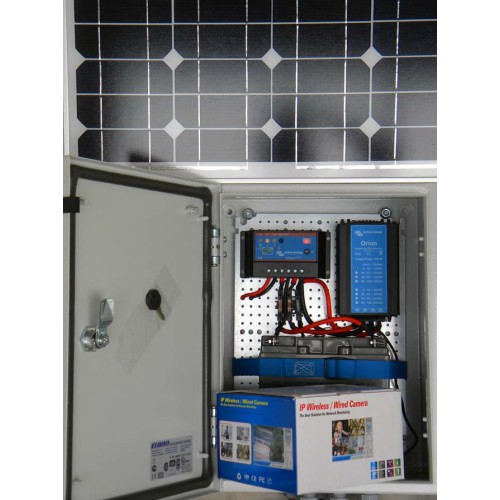
\includegraphics[width=50mm]{img/conception/electrosun_cam.jpg}
    \centering
    \captionsource{\textbf{Electrosun} Caméra de surveillance solaire}{\autocite{cam:electrosun_site}}
\end{figure}

Bien qu'elle satisfasse la plupart des contraintes, elle n'a pas été retenue pour l'évaluation. En effet, la résolution des images capturées n'est que de 640x480 pixels, ce qui n'est pas suffisant.

\paragraph{\textbf{Reolink} -- Argus 2}
L'entreprise \textit{Reolink} développe des caméras 100\% sans fil, avec batteries rechargeables et panneaux solaires. Elle est auto-suffisante.\autocite{cam:argus2}

\begin{figure}[h]
    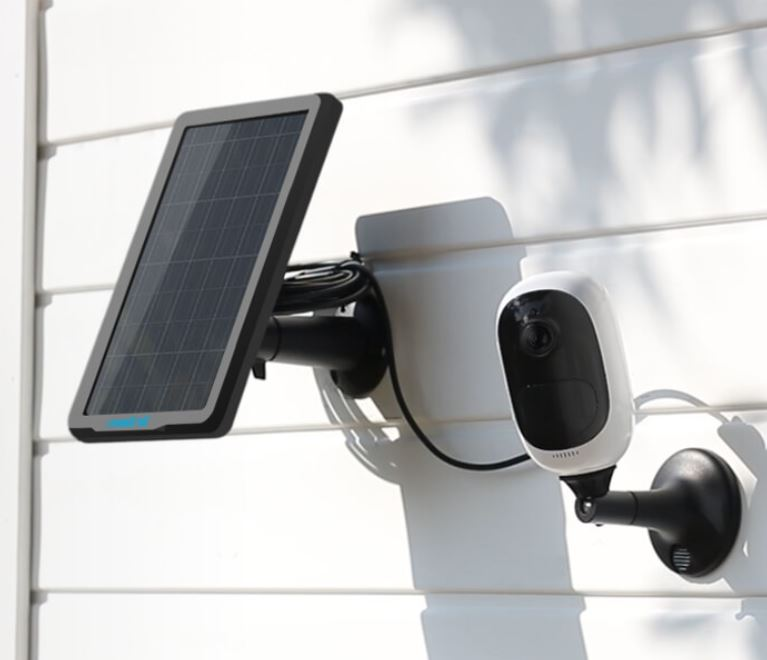
\includegraphics[width=50mm]{img/conception/argus2_cam.jpg}
    \centering
    \captionsource{\textbf{Reolink} Argus 2}{\autocite{cam:argus2}}
\end{figure}

Elle permet de capturer des photos FullHD (1920x1080 pixels), possède une fonction de vision de nuit ou encore, l'utilisation en extérieur est possible. Cependant, cette caméra n'a elle non plus pas pu être prise en considération. En effet, elle a été pensée pour un usage privé, et bien que la caméra puisse être connectée à un réseau Wifi, l'accès à celle-ci n'est possible qu'à l'aide d'une application smartphone (tel que décrit dans les spécifications disponibles sur le site officiel \url{https://reolink.com/product/argus-2}\autocite{cam:argus2}). Récupérer des photographies à intervalles réguliers semble donc difficilement réalisable.

\paragraph{\textbf{Wanscam} -- HW0029-3}

\textit{Wanscam} est une entreprise chinoise spécialisées dans la production de caméra réseau. Plusieurs versions de son modèle \textit{HW0029} sont disponibles. Ici est présenté le modèle \textit{HW0029-3}. \autocite{cam:wan3}

\begin{figure}[h]
    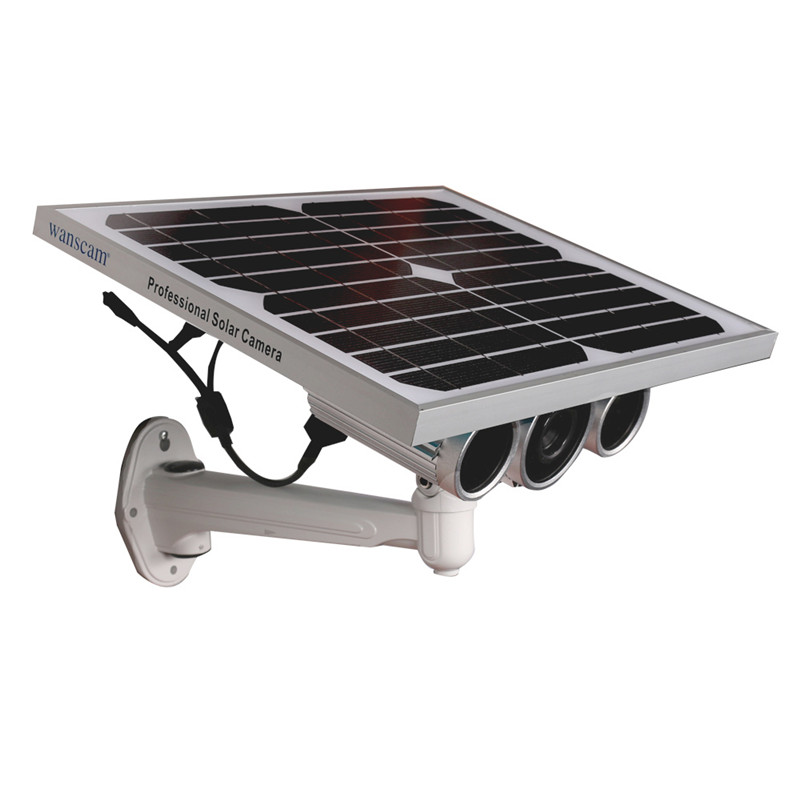
\includegraphics[width=50mm]{img/conception/wan3_cam.jpg}
    \centering
    \captionsource{\textbf{Wanscam} HW0029-3}{\autocite{cam:wan3}}
\end{figure}

Cette caméra satisfait toutes les contraintes définies en section \ref{conception.techno.camera.contraintes}. On trouvera en table \ref{tab:HW0029-3} ses principales caractéristiques.\footnote{Tirées des spécifications officielles \autocite{cam:wan3} et d'un test indépendant \autocite{cam:wan3-test}}

\begin{table}[!h]
    \centering
    \caption{Caractéristiques de la caméra \textbf{Wanscam} \textit{HW0029-3}}
    \label{tab:HW0029-3}
    \begin{tabular}{@{}ll@{}}
    \toprule
    Caractéristique        & Valeurs                                                                                                                                                                                                                                                                                     \\ \midrule
    Image                  & 1280 x 720, 25fps, compression H.264                                                                                                                                                                                                                                                        \\
    Angle de vue           & 40°                                                                                                                                                                                                                                                                                         \\
    Vision nocture         & Visibilité jusqu'à 15 mètres                                                                                                                                                                                                                                                                \\
    Réseau                 & RJ45, WiFi 802.11 b/g/n                                                                                                                                                                                                                                                                     \\
    Auto-alimentation      & \begin{tabular}[c]{@{}l@{}}2 batteries de 12A et panneau solaire. \\ Sans soleil: 48h d'utilisation. \\ Faible température (\textless 26°) des rayons de soleil: 7 jours d'utilisations. \\ Grande température (\textgreater 33°) des rayons de soleil: fonctionnement continu\end{tabular} \\
    Stockage               & Carte MicroSD de 16Gb incluse, support jusqu'à 128Gb                                                                                                                                                                                                                                        \\
    Détection de mouvement & Oui                                                                                                                                                                                                                                                                                         \\
    Accès aux images       & Flux HTTP, ONVIF, RTSP, requêtes HTTP                                                                                                                                                                                                                                                       \\
    Dimensions et poids    & 370x290x110 mm, 2.7 kg                                                                                                                                                                                                                                                                      \\ \bottomrule
    \end{tabular}
\end{table}

On notera que le panneau solaire est fixé sur la caméra. Ainsi, dans le but de garder une exposition au soleil suffisante, l'angle de la caméra ne doit pas être trop élevé. Il y a donc certaines contraintes à l'installation de celle-ci.

Concernant la capture d'image, la caméra fournit des \textit{endpoints HTTP} (dont une liste peut être trouvée sur le site \url{tutoriels.domotique-store.fr}\autocite{cam:wan3-url}) permettant de récupérer l'image actuelle. Il est donc facile d'imaginer un simple agent qui, à intervalle régulier, demandera à la caméra une image, et l'enregistrera en local.

Les caméras \textbf{Wanscam} ne sont pas des plus faciles à trouver dans le commerce. Elles sont principalement disponibles sur \url{aliexpress.com}. Le modèle \textit{HW0029-3} peut être trouvé à partir de 170CHF (en date du 09.03.2018).

La grille d'évaluation \ref{cam:wan3_eval} a pu être remplie à l'aide des différents critères.

\begin{table}[!h]
    \centering
    \caption{Evaluation de la caméra \textbf{Wanscam} \textit{HW0029-3}}
    \label{cam:wan3_eval}
    \begin{tabular}{@{}llp{8cm}@{}}
        \toprule
        Critère                              & Note (de 1 à 5) & Remarque                                                                                                                                                                   \\ \midrule
        Qualité d'image              & 3 [1]               & La qualité d'image semble suffisante selon les tests effectué par \url{lesbonstuyauxgeeks.fr}\autocite{cam:wan3-test}.                                                                                                              \\
        Fonctionnalités réseaux      & 5 [2]              & La caméra offre notamment un endpoint HTTP sur lequel récupérer les images.                                                                                                \\
        Fonctionnement auto-alimenté & 4 [4]              & La caméra est totalement auto-suffisante s'il y a assez de soleil. On notera cependant le panneau solaire fixe qui peut nuire à l'exposition du soleil.                    \\
        Capture de photo             & 5 [2]              & Il est facile de récupérer des images sur cette caméra. Elle offre en plus un système de capture de photos à intervalles réguliers automatique.                            \\
        Angle de vue                 & 1 [2]              & Un angle de vue de 40° semble tout juste suffisant.                                                                                                                        \\
        Vision de nuit               & 2 [1]               & Elle fournit une vision nocturne à 15m. Il est cependant possible d'ajouter des LEDs infrarouges supplémentaires afin d'obtenir une meilleure vision de nuit\autocite{cam:wan3-url}. \\
        Facilité d'installation      & 3 [1]              & La caméra mesure jusqu'à 37 cm, ce qui nuit à sa facilité d'installation. De plus, le panneau solaire est fixe, ce qui contraint la position et l'angle de la caméra.      \\
        Prix                         & 4 [2]              & A partir d'environ 170.- CHF \\ \bottomrule
        && \textbf{Note finale: 3.86}
    \end{tabular}
\end{table}

\subsubsection{Evaluation}
